\documentclass{article}


% ready for submission
% \usepackage{neurips_2024}
% \usepackage[preprint]{neurips_2024}
\usepackage{iclr2025_conference}

\usepackage{graphicx} 
\usepackage[utf8]{inputenc} % allow utf-8 input
\usepackage[T1]{fontenc}    % use 8-bit T1 fonts
\usepackage{hyperref}       % hyperlinks
\usepackage{url}            % simple URL typesetting
\usepackage{booktabs}       % professional-quality tables
\usepackage{amsfonts}       % blackboard math symbols
\usepackage{nicefrac}       % compact symbols for 1/2, etc.
\usepackage{microtype}      % microtypography
\usepackage{xcolor}         % colors
\usepackage{wrapfig}
\usepackage{subcaption}
\usepackage{multirow}
\usepackage{multicol}
\usepackage{array}
\usepackage[usestackEOL]{stackengine}
\usepackage{xspace}
\usepackage{amsmath}
\usepackage{cleveref}
\usepackage[most]{tcolorbox}
\usepackage{minitoc}
\usepackage{appendix}
\usepackage{titletoc}
\usepackage{float}
 
\newcommand{\hide}[1]{}

\newcommand{\model}{CogVideoX\xspace} 
\newcommand{\dong}[1]{\textbf{\color{red}[(Dong: #1 )]}}
\newcommand{\gxt}[1]{\textbf{\color{cyan}[Gu: #1 ]}}

\newcommand{\fix}{\marginpar{FIX}}
\newcommand{\new}{\marginpar{NEW}}

\newcommand{\aspace}{\hspace{1em}}

\newtcolorbox{promptbox}[1][]{
  breakable,
  title=#1,
  colback=gray!5,
  colframe=black,
  colbacktitle=gray!15,
  coltitle=black,
  fonttitle=\bfseries,
  bottomrule=1.5pt,
  toprule=1.5pt,
  leftrule=1pt,
  rightrule=1pt,
  arc=0pt,
  outer arc=0pt,
  enhanced,
  before upper={\parindent=1.5em}
}


% author formatting
\usepackage{authblk}
\renewcommand\Authands{, } %
\renewcommand{\Authfont}{\bfseries}
\makeatletter
\renewcommand\AB@affilsepx{, \protect\Affilfont}
\makeatother

\title{
\includegraphics[width=0.07\textwidth]{images/logo.png}
CogVideoX: Text-to-Video Diffusion Models with An Expert Transformer}

\author{Zhuoyi Yang$^{\star}$ \aspace  Jiayan Teng$^{\star}$ \aspace  Wendi Zheng  \aspace Ming Ding \aspace  Shiyu Huang \\ 
Jiazheng Xu \aspace
Yuanming Yang\aspace  Wenyi Hong\aspace  Xiaohan Zhang \aspace Guanyu Feng  \\ 
Da Yin  
\aspace Xiaotao Gu  \aspace  Yuxuan Zhang \aspace Weihan Wang  \aspace Yean Cheng \\ Ting Liu \aspace   Bin Xu \aspace  
  Yuxiao Dong \aspace  Jie Tang \\
~\\ 
\textnormal{Zhipu AI \aspace Tsinghua University}
}
% \affil[]{Zhipu AI \aspace Tsinghua University}
\affil[]{}


%  \hide{
% \author{Zhuoyi Yang$^{\star}$ \aspace {\bf Jiayan Teng}$^{\star}$ \aspace {\bf Wendi Zheng} \aspace {\bf Ming Ding} \aspace {\bf Shiyu Huang} \\
% \aspace {\bf Jiazheng Xu} \aspace
% {\bf Yuanming Yang} \aspace {\bf Xiaohan Zhang} \aspace {\bf Xiaotao Gu} \aspace  {\bf Guanyu Feng}\aspace \\
%  {\bf Da Yin} 
% \aspace {\bf Wenyi Hong} \aspace  {\bf Weihan Wang} \aspace
%  {\bf Yean Cheng} \aspace {\bf Yuxuan Zhang} \aspace  \\
%  {\bf Ting Liu} \aspace {\bf Bin Xu}  \aspace {\bf Yuxiao Dong} \aspace {\bf Jie Tang}~\\
% $^{1}$Zhipu AI \aspace $^{2}$Tsinghua University\\
% \textmd{\href{https://github.com/THUDM/CogVideo}{https://github.com/THUDM/CogVideo}} 
% }
% }

% $^1$Zhipu AI\ \ \ \ \ \ $^2$Tsinghua University 
% \href{https://github.com/THUDM/CogVideo}{https://github.com/THUDM/CogVideo}
 
% \newcommand{\yzy}{\textcolor{red}{\textbf{ZHUOYI}}}
% \newcommand{\tjy}{\textcolor{red}{\textbf{JIAYAN}}}
\newcommand{\anonymous}{{\textit{Anonymous}}}

\iclrfinalcopy % Uncomment for camera-ready version, but NOT for submission.\begin{document}

\begin{document}


\maketitle

\renewcommand{\thefootnote}{}
\footnotetext{*Equal contributions. Core contributors: Zhuoyi, Jiayan, Wendi, Ming, and Shiyu.}
\footnotetext{{\{yangzy22,tengjy24\}@mails.tsinghua.edu.cn, \{yuxiaod,jietang\}@tsinghua.edu.cn}}
\footnotetext[1]{Visiting our demo website \href{https://yzy-thu.github.io/CogVideoX-demo/}{demo} to watch more generated videos!}
\renewcommand{\thefootnote}{\arabic{footnote}}

% \footnotemark[1]

\begin{figure}[ht]
\vspace{-10mm}
\centering
\includegraphics[width=\textwidth]{images/front.jpg}
\caption{
CogVideoX can generate long-duration, high-resolution videos with coherent actions and rich semantics.}
\label{fig:exampleImage}
\end{figure}

\begin{abstract}
%  Previous video generation models often had limited movement and short durations, making it difficult to generate videos with coherent narratives based on text. We propose several designs to address these issues and, train the CogVideoX., 
% To efficently model video data, we propose to levearge a 3D Variational Autoencoder (VAE) to compress videos along both spatial and temporal dimensions. 
% To improve the text-video alignment, we propose an expert transformer with the expert adaptive LayerNorm to facilitate the deep fusion between the two modalities. 
% By employing a progressive training technique, \model is adept at producing coherent, long-duration videos characterized by significant motions. 
% In addition, we develop an effective text-video data processing pipeline that includes various data preprocessing strategies and a video captioning method. 
% It significantly helps enhance the performance of \model, improving both generation quality and semantic alignment. 
% We introduce \model, large-scale diffusion transformer models designed for generating videos based on text prompts.

% Results show that \model demonstrates state-of-the-art performance across both multiple machine metrics and human evaluations. 
% The model weights of both the 3D Causal VAE and \model are publicly available at \anonymous.
%\url{https://github.com/THUDM/CogVideo}. 
% and \url{https://huggingfaces.co/THUDM/CogVideoX}. 

% Previous video generation models often had limited movement and short durations, making it difficult to generate videos with coherent narratives based on text. We propose several designs to address these issues and, introduce \model, large-scale diffusion transformer models which can generate 768$\times$ 1360 at 16 fps, 10 seconds videos based on text prompts. 
% First, we propose to levearge a 3D Variational Autoencoder (VAE) to compress videos along both spatial and temporal dimensions. Second, to improve the text-video alignment, we propose an expert transformer with the expert adaptive LayerNorm to facilitate the deep fusion between the two modalities. Third, by employing a progressive training and multi-resolution frame pack technique, \model is adept at producing coherent, long-duration, different shape videos characterized by significant motions. 
% In addition, we develop an effective text-video data processing pipeline that includes various data preprocessing strategies and a video captioning method. 
% It significantly helps enhance the performance of \model, improving both generation quality and semantic alignment. 
% Results show that \model demonstrates state-of-the-art performance across both multiple machine metrics and human evaluations. 
% The model weights of both the 3D Causal VAE and \model are publicly available at \anonymous.

We present \model, a large-scale text-to-video generation model based on diffusion transformer, which can generate 10-second continuous videos aligned with text prompt, with a frame rate of 16 fps and resolution of 768$\times$ 1360 pixels. 
Previous video generation models often had limited movement and short durations, and is difficult to generate videos with coherent narratives based on text. We propose several designs to address these issues. 
First, we propose a 3D Variational Autoencoder (VAE) to compress videos along both spatial and temporal dimensions, to improve both compression rate and video fidelity. Second, to improve the text-video alignment, we propose an expert transformer with the expert adaptive LayerNorm to facilitate the deep fusion between the two modalities. Third, by employing a progressive training and multi-resolution frame pack technique, \model is adept at producing coherent, long-duration, different shape videos characterized by significant motions. 
In addition, we develop an effective text-video data processing pipeline that includes various data preprocessing strategies and a video captioning method,
% . It significantly helps enhance the performance of \model, improving both generation quality and semantic alignment. 
greatly contributing to the generation quality and semantic alignment. 
Results show that \model demonstrates state-of-the-art performance across both multiple machine metrics and human evaluations. 
% The model weights of the 3D Causal VAE, the video caption model, and CogVideoX are open-source.
The model weight of both 3D Causal VAE, Video caption model and \model are publicly available at \href{https://github.com/THUDM/CogVideo}{https://github.com/THUDM/CogVideo}.


\end{abstract}


\section{Introduction}
\label{sec:introduction}

\begin{wrapfigure}{r}{0.5\textwidth}
\vspace{-6mm}
\begin{center}
    \includegraphics[width=0.5\textwidth]{images/cover.pdf}
  \end{center}
  \vspace{-4mm}
  \caption{\textbf{Overview of \implname.} In training, we tune the singular values of the weight matrices to generate a set of ``expert'' vectors specializing in different tasks. In inference, a two-pass process is adopted where the first applies the expert and the second generates the answer.}
  \label{fig:cover}
  \vspace{-4mm}
\end{wrapfigure}

Self-adaptive large language models (LLMs) would represent a significant advancement in artificial intelligence, enabling real-time adaptation to various tasks and contexts.
While compositionality and scalability are crucial for effective adaptation, current LLM training methodologies fall short of achieving both these properties simultaneously.
Our research aims to present a solution to address these gaps.

In principle, the first step toward achieving self-adaptive LLMs can be realized through the development of specialized expert modules, each fine-tuned~\citep{kaplan2020scaling} via techniques such as low-rank adaptation (LoRA)~\citep{hu2021lora}. 
However, several challenges need to be addressed to make this approach both scalable and compositional: (1) multiple expert modules significantly increase the number of parameters; (2) expert modules are often prone to overfitting; and (3) flexible composition of these experts is still an open problem.

To overcome these limitations, we first propose \svdacro, a novel parameter-efficient fine-tuning (PEFT) method to obtain effective building blocks for self-adaptation.
\svdacro works by extracting and selectively tuning only the singular values within the model's weight matrices.
By focusing on this essential and principled parameterization, our approach mitigates the risk of overfitting, drastically reduces computational demands, and allows for inherent compositionality.

We then introduce our full \implname framework, which entails a two-pass inference mechanism to produce dynamically adapted weights targeted for the test-time conditions (Figure~\ref{fig:cover}).
We design three different adaptation strategies that can be used within \implname, which we show provide monotonic performance benefits with increasing access to the test-time conditions.
We evaluate \svdacro and the full \implname framework through extensive experiments across a diverse range of LLMs and tasks.
\svdacro outperforms traditional efficient fine-tuning methods like LoRA on domain-specific datasets with far fewer parameters. 
\implname further improves performance, even for out-of-distribution tasks like visual QA. 
Our analysis even shows that \implname allows the reuse of \svdacro experts across different LLMs. In summary, our key technical contributions are: 
\vspace{-2mm}
\begin{itemize}
\item The development of \implname as a pivotal self-adaptation framework for LLMs, providing a blueprint to adapt the behavior of LLMs from a growing set of pre-trained skills.
\item The introduction of \svdacro, a novel PEFT method trainable with RL on small datasets, producing compact expert vectors with inherent compositionality.
\item The implementation of three adaptation strategies, effectively dispatching \svdacro-trained experts with properties designed to cope with different deployment scenarios.
\end{itemize}

\vspace{-2mm}
\subsection{3D Variational Auto-encoder Design}\label{3dVAE}

Similar to previous work~\cite{polyak2024movie,yang2024cogvideox}, we train a 3DVAE to compress pixel-space videos and images into a compact latent space. To handle both videos and images, we adopt CausalConv3D~\cite{yu2023language}. For a video of shape $(T+1) \times 3 \times H \times W$, our 3DVAE compresses it into latent features with shape $(\frac{T}{c_t} + 1) \times C \times (\frac{H}{c_s}) \times (\frac{W}{c_s})$. In our implementation, $c_t=4$, $c_s=8$, and $C=16$. This compression significantly reduces the number of tokens for the subsequent diffusion transformer model, allowing us to train videos at the original resolution and frame rate. The model structure is illustrated in Figure \ref{fig:vae-model-arch}.

\begin{figure}[t]
    \centering
    \includegraphics[width=0.95\linewidth]{figures/vae-model-arch.pdf}
    \caption{ The architecture of our 3DVAE.}
    \label{fig:vae-model-arch}
\end{figure}

\subsubsection{Training}
In contrast to most previous work \cite{polyak2024movie,chen2024od,zhou2024allegro}, we do not rely on a pre-trained image VAE for parameter initialization; instead, we train our model from scratch. 
To balance the reconstruction quality of videos and images, we mix video and image data at a ratio of $4:1$. Besides the routinely used $L_1$ reconstruction loss and KL loss $L_{kl}$, we also incorporate perceptual loss $L_{lpips}$ and GAN adversarial loss $L_{adv}$ \cite{esser2021taming} to enhance the reconstruction quality. The complete loss function is shown in Equation \ref{eq:vae-loss}.

\begin{equation}
    \label{eq:vae-loss}
    \text{Loss} = L_{1} + 0.1 L_{lpips} + 0.05 L_{adv} + 10^{-6} L_{kl}
\end{equation}

During training, we employ a curriculum learning strategy, gradually training from low-resolution short video to high-resolution long video. To improve the reconstruction of high-motion videos, we randomly choose a sampling interval from the range $1 \sim 8$ to sample frames evenly across video clips.

\subsubsection{Inference}
Encoding and decoding high-resolution long videos on a single GPU can lead to out-of-memory (OOM) errors. To address this, we use a spatial-temporal tiling strategy, splitting the input video into overlapping tiles along the spatial and temporal dimensions. Each tile is encoded/decoded separately, and the outputs are stitched together. For the overlapping regions, we utilize a linear combination for blending. This tiling strategy allows us to encode/decode videos in arbitrary resolutions and durations on a single GPU.

We observed that directly using the tiling strategy during inference can result in visible artifacts due to inconsistencies between training and inference. To solve this, we introduce an additional finetuning phase where the tiling strategy is randomly enabled/disabled during training. This ensures the model is compatible with both tiling and non-tiling strategies, maintaining consistency between training and inference. 

\begin{figure}[ht]
    \centering
    \ifhq
    \includegraphics[width=\linewidth]{hqfigures/vae-sota-cmp.png}
    \else
    \includegraphics[width=\linewidth]{figures/vae-sota-cmp.pdf}
    \fi
    \caption{VAE reconstruction case comparison.}
    \label{fig:vae-sota-cmp}
\end{figure}

Table \ref{tab:sota_vae} compares our VAE with open-source state-of-the-art VAEs. On video data, our VAE demonstrates a significantly higher PSNR compared to other video VAEs. On images, our performance surpasses both video VAEs and image VAE. Figure \ref{fig:vae-sota-cmp} shows several cases at $256 \times 256$ resolution. Our VAE demonstrates significant advantages in text, small faces, and complex textures.
%Table \ref{tab:sota_vae} compares our VAE with open-source state-of-the-art VAEs. On video data, our VAE demonstrates a significantly higher PSNR compared to other video VAEs, achieving performance comparable to frame-wise image VAE while maintaining a 4x higher temporal compression. On images, our PSNR not only surpasses that of other video VAEs but also exceeds that of image VAE. Figure \ref{fig:vae-sota-cmp} shows several cases at $256 \times 256$ resolution. It is evident that our VAE demonstrates significant advantages in  text, small faces, and complex textures.


\begin{table*}[ht]
\renewcommand{\arraystretch}{1.2}
\small
\centering  
\caption{VAE reconstruction metrics comparison.}
\begin{tabular}{lcccc}
\toprule
\multirow{2}{*}{Model} & Downsample  & \multirow{2}{*}{$|z|$} & ImageNet (256$\times$256)
& MCL-JCV (33$\times$360$\times$640) \\
& Factor & & PSNR$\uparrow$ & PSNR$\uparrow$ \\
\midrule
%FLUX-VAE~\cite{FLUX}                   & $1 \times 8 \times 8$ & 16 & 32.70 & 37.87 \\
FLUX-VAE~\cite{FLUX}                   & $1 \times 8 \times 8$ & 16 & 32.70 & - \\
\midrule
OpenSora-1.2~\cite{opensora}           & $4 \times 8 \times 8$ & 4  & 28.11 & 30.15 \\
CogvideoX-1.5~\cite{yang2024cogvideox} & $4 \times 8 \times 8$ & 16 & 31.73 & 33.22 \\
Cosmos-VAE~\cite{cosmos}               & $4 \times 8 \times 8$ & 16 & 30.07 & 32.76 \\
Ours                                   & $4 \times 8 \times 8$ & 16 & 33.14 & 35.39 \\
\bottomrule
\end{tabular}
\label{tab:sota_vae}
\end{table*}

\subsection{Overall Pipeline}
\label{sec:overall}
Fig.\ref{fig:refiner}(a) presents the proposed Apollo pipeline. Apollo operates in the time-frequency domain and comprises a band-split module, a band-sequence modeling module, and a band-reconstruction module. Specifically, given compressed or distorted audio $\mathbf{S}\in \mathbb{R}^{1\times L}$, we first transfer $\mathbf{S}$ to its time-frequency domain representation $\mathbf{X}\in \mathbb{C}^{F\times T}$ using the Short-Time Fourier Transform (STFT), where $L$ denotes the length of audio, $F$ and $T$ denote the number of frequency bins and frames, respectively. Then, the band-split module maps to sub-band embeddings $\mathbf{Z}\in \mathbb{R}^{N\times T}$ using gain-shape representations $\mathbf{G}\in \mathbb{R}^{3\times M\times T}$ for each sub-band, where $N$ and $M$ denote the number of channels in sub-band embeddings and gain-shape representations, respectively. Next, the band-sequence modeling module performs joint modeling of temporal and sub-band using a stacked architecture based on Roformer \cite{su2024roformer} and temporal convolutional network (TCN) \cite{bai2018empirical,li2022efficient}. Finally, the band-reconstruction module converts the output $\mathbf{Q}\in \mathbb{R}^{N\times T}$ of the band-sequence modeling module into the reconstructed complex-valued spectrogram $\mathbf{Y}\in \mathbb{C}^{F\times T}$. It uses the inverse Short-Time Fourier Transform (iSTFT) to convert $\mathbf{Y}$ to a waveform $\bar{\mathbf{S}}\in \mathbb{R}^{1\times L}$.

\begin{table*}[]
\footnotesize
\centering
\caption{The structure of the STFT discriminator network.}
\begin{tabular}{cccccccc}
\toprule
\textbf{Layer Index} & \textbf{Layer Type}   & \textbf{Input Channels} & \textbf{Output Channels} & \textbf{Kernel Size} & \textbf{Padding} & \textbf{Stride} & \textbf{Activation} \\ \midrule
1                    & SpectralNorm + Conv2d & $F$                       & $F$                        & (3, 3)               & (1, 1)           & (1, 1)          & LeakyReLU(0.2)      \\
2                    & SpectralNorm + Conv2d & $F$                       & $F\times 2$              & (3, 3)               & (1, 1)           & (2, 2)          & LeakyReLU(0.2)      \\
3                    & SpectralNorm + Conv2d & $F\times 2$             & $F\times 4$              & (3, 3)               & (1, 1)           & (1, 1)          & LeakyReLU(0.2)      \\
4                    & SpectralNorm + Conv2d & $F\times 4$             & $F\times 8$              & (3, 3)               & (1, 1)           & (2, 2)          & LeakyReLU(0.2)      \\
5                    & SpectralNorm + Conv2d & $F\times 8$             & $F\times 16$             & (3, 3)               & (1, 1)           & (1, 1)          & LeakyReLU(0.2)      \\
6                    & SpectralNorm + Conv2d & $F\times 16$            & $F\times 32$             & (3, 3)               & (1, 1)           & (2, 2)          & LeakyReLU(0.2)      \\
7                    & Conv2d                & $F\times 32$            & 1                        & (3, 3)               & (1, 1)           & (1, 1)          & None               \\ \bottomrule
\end{tabular}
\label{tab:dis}
\vspace{-10pt}
\end{table*}

\subsection{Band-split Module}
As shown in Fig.\ref{fig:refiner}(b), given compressed or distorted audio spectrogram $\mathbf{X}$, we first split its frequency dimension $F$ into $K$ sub-band spectrograms $\{\mathbf{X}_k\in \mathbb{C}^{M_k\times T} | k\in [1, K]\}$. Inspired by the Gull codec \cite{luo2024gull}, we extract gain-shape representations $\mathbf{G}_k\in \mathbb{R}^{3\times M_k\times T}$ for each sub-band spectrogram:
\begin{equation}
\begin{aligned}
\mathbf{G}_{k} = \operatorname{Concat} \left[ 
\frac{\operatorname{Re}(\mathbf{X}_{k})}{\|\mathbf{X}_{k}\|_2}, \ 
\frac{\operatorname{Im}(\mathbf{X}_{k})}{\|\mathbf{X}_{k}\|_2}, \ 
\log\left(\|\mathbf{X}_{k}\|_2\right),
\right]
\end{aligned}
\end{equation}
where $\operatorname{Re}(\mathbf{X}_{k})$ and $\operatorname{Im}(\mathbf{X}_{k})$ denote the real and imaginary parts, respectively. $\|\mathbf{X}_{k}\|_2$ represents the $\ell_2$-norm of $\mathbf{X}_{k}$, given by:
\begin{equation}
    \|\mathbf{X}_{k}\|_2 = \sqrt{\operatorname{Re}(\mathbf{X}_{k})^2 + \operatorname{Im}(\mathbf{X}_{k})^2}
\end{equation}
$\log\left(\|\mathbf{X}_{k}\|_2\right)$ is the logarithm of the $\ell_2$-norm of $\mathbf{X}_{k}$. $\operatorname{Concat}$ refers to the concatenation of components. The gain-shape representation decouples the sub-band spectrogram's content and energy, allowing the reconstruction model to learn appropriate mappings that preserve the audio content. Subsequently, we map the gain-shape representations $\mathbf{G}$ into high-dimensional embeddings $\mathbf{Z}$ through a bottleneck layer, which consists of RMSNorm \cite{zhang2019root} and a 1D convolutional layer.

\subsection{Band-sequence Modeling Module}
In Apollo, we employ stacked Band-sequence modeling modules (BS modules, Fig.\ref{fig:refiner}(c)) to perform joint sub-band and temporal modeling with a stacking depth of $B$. Unlike BSRNN \cite{luo2023music} and Gull \cite{luo2024gull}, each BS module consists of a series of residual Roformers \cite{su2024roformer} and TCNs, which sequentially scan along the sub-band and time dimensions, and can increase the modeling capacity to improve the model performance. First, the residual Roformer is applied to the input $\mathbf{Z}$ along the frequency band dimension $K$ to obtain $\mathbf{Z}'\in \mathbb{R}^{N\times T}$, capturing global dependencies between sub-bands while preserving the local characteristics of the frequency domain signals. Next, the TCN is applied along the time dimension $T$ on $\mathbf{Z}'$ to generate the output $\mathbf{Q}\in \mathbb{R}^{N\times T}$. Since the $K$ sub-band features share the same feature dimension $N$, they all share a single TCN. The TCN consists of three convolutional blocks, each containing three convolutional layers. This design allows the TCN module to efficiently handle short-term dependencies and local temporal dynamics in audio signals, enhancing the model's ability to capture and understand temporal domain features.

\subsection{Band-reconstruction Module}
The output $\mathbf{Q}$ is passed through sub-band-specific fully connected (FC) layers to generate the estimated real and imaginary parts of the restored sub-band spectrograms (see Fig.\ref{fig:refiner}(d)). We utilize RMSNorm as the normalization layer within the fully connected layers and employ Gated Linear Units (GLUs) as the nonlinear activation function. Subsequently, the $K$ reconstructed sub-band spectrograms are concatenated along the frequency dimension to form the final reconstructed complex-valued spectrogram $\mathbf{Y}$. Finally, the reconstructed complex-valued spectrogram $\mathbf{Y}$ is converted back to the waveform domain $\bar{\mathbf{S}}$ through the iSTFT.

\begin{figure*}[h]
	\small
	\centering
	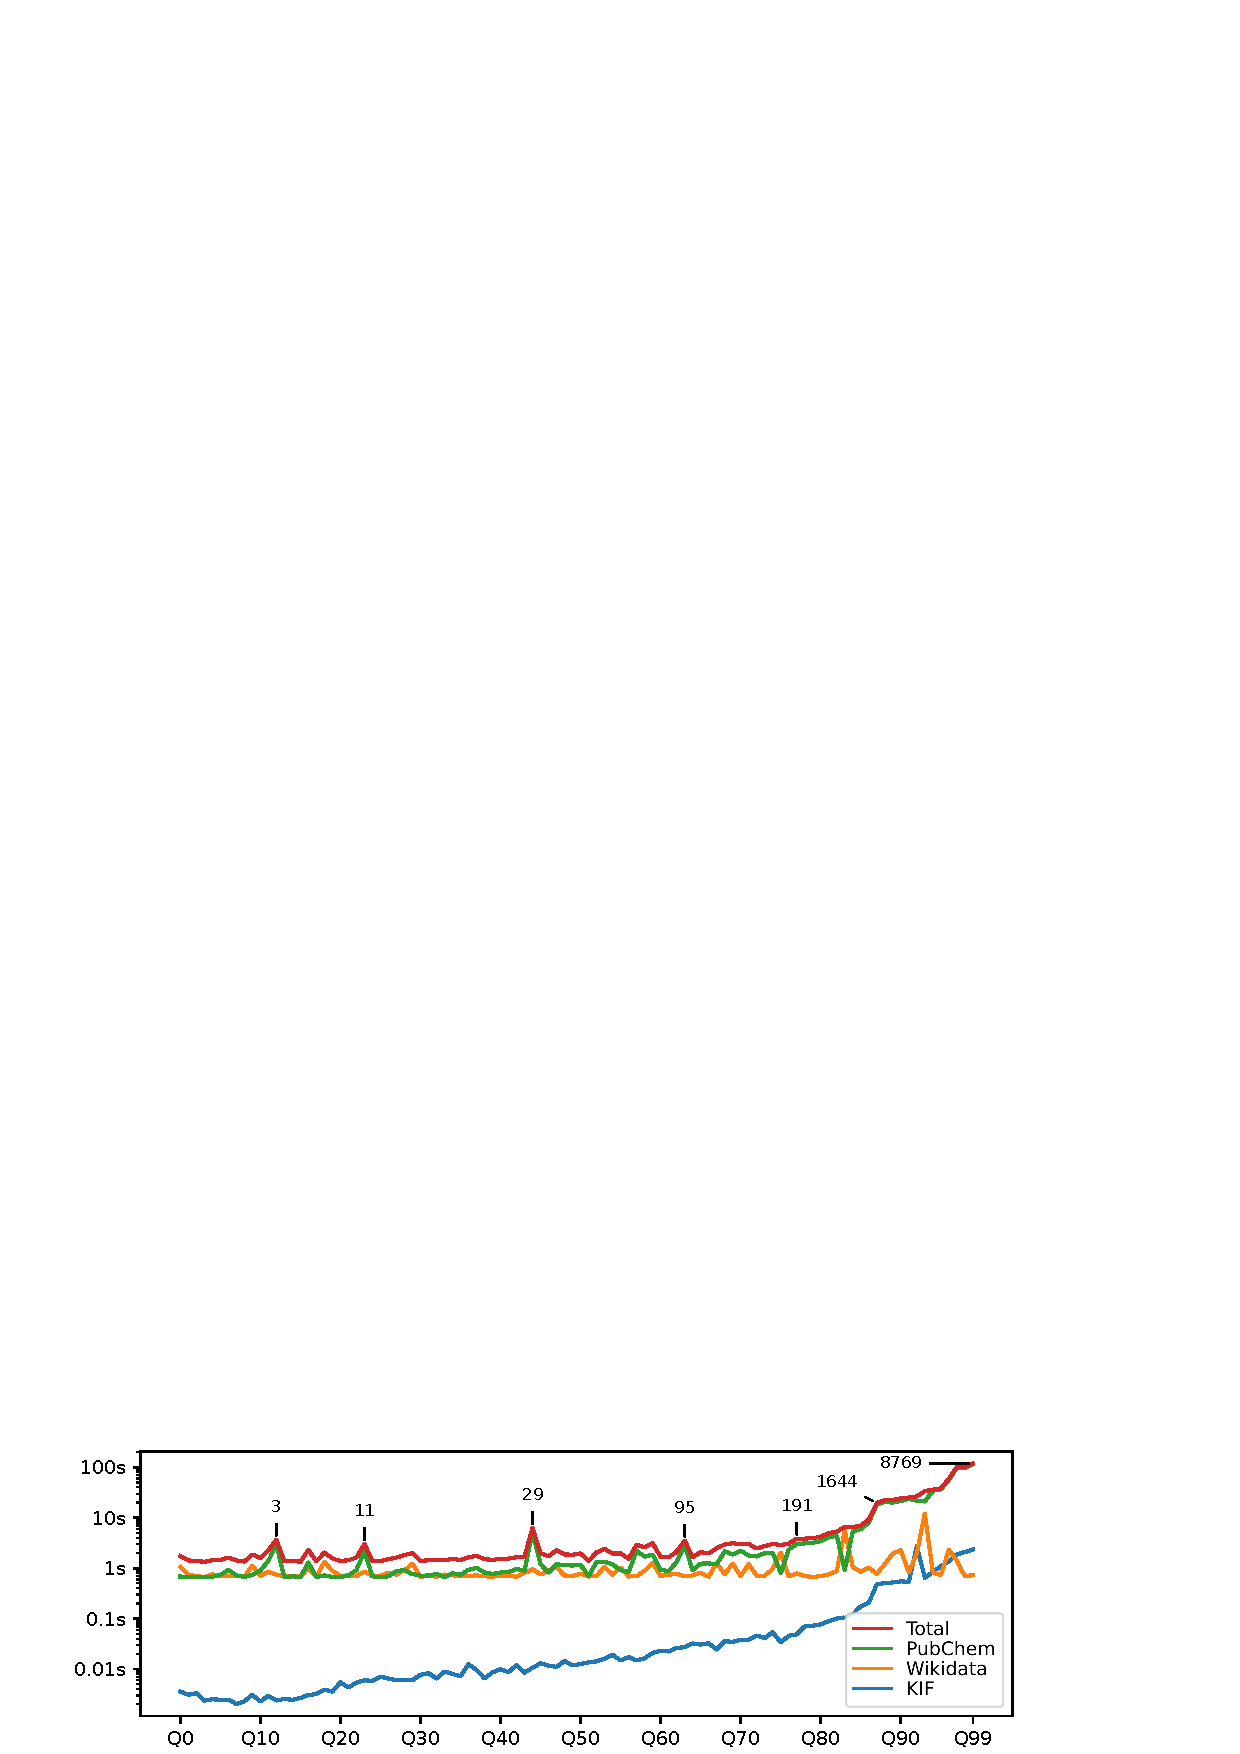
\includegraphics[width=2.0\columnwidth]{Figures/plot.pdf}
	\caption{Apollo and SR-GAN's SDR, SI-SNR and ViSQOL result in comparison at different bitrates.}
	\label{fig:plot}
\end{figure*}

\begin{table*}[]
\footnotesize
\centering
\caption{Different methods' SDR/SI-SNR/VISQOL scores for various types of music, as well as the number of model parameters and GPU inference time. For the GPU inference time test, a music signal with a sampling rate of 44.1 kHz and a length of 1 second was used.}
\begin{tabular}{cccccccc}
\toprule
Model  & Vocal            & Single Stem      & Multi-Stems      & Multi-Stems+Vocal & Overall   & Params (M) & RTF (ms)      \\ \midrule
SR-GAN \cite{lattner2021stochastic} & 10.62/9.19/2.72  & 13.88/12.52/3.28 & 14.92/14.16/3.41 & 16.87/15.54/3.76  & 14.07/12.85/3.29 & 322.53 & \textbf{34.55}\\
Apollo (Ours) & \textbf{13.99/12.58/3.44} & \textbf{16.56/15.99/4.08} & \textbf{17.52/17.15/4.41} & \textbf{18.51/18.26/4.54}  & \textbf{16.64/16.00/4.12} & \textbf{16.54} & 53.23 \\ \bottomrule
\end{tabular}
\label{tab:stems}
\vspace{-10pt}
\end{table*}

\subsection{Training Objection}
The proposed Apollo model is trained using a GAN framework to enhance the quality of audio restoration. Specifically, the discriminator network is inspired by the multi-resolution STFT discriminator, similar to the Gull codec \cite{luo2024gull}. As described in Table \ref{tab:dis}, the discriminator input consists of the spectrogram's real and imaginary parts, which are stacked into a 3D tensor along the channel dimension. To ensure energy invariance in the input, the signal is normalized to have a unit $\ell_2$-norm before being passed into the discriminator. The discriminator is trained using the Least Squares GAN (LSGAN) loss \cite{mao2017least}, defined as:
\begin{equation}
    L_{\text{D}} = \sum_{i=1}^{I}\mathbb{E}_{\mathbf{A} \sim p_{\text{data}}} \left[ (D_i(\mathbf{A}) - 1)^2 \right] + \sum_{i=1}^{I}\mathbb{E}_{\mathbf{Y} \sim p_{\text{G}}} \left[ (D_i(\mathbf{Y}))^2 \right],
\end{equation}
where $\mathbf{A}\in \mathbb{C}^{F\times T}$ denotes the spectrogram of uncompressed audio and $I=5$ denotes the number of discriminator. 

The generator, Apollo, is optimized through a composite loss function, which includes the reconstruction loss, feature matching loss, and the adversarial loss from the discriminator. The \textit{reconstruction loss} $L_{\text{rec}}$ is based on the mean absolute error (MAE) between the magnitude spectrograms of the restored and target audio, evaluated over multiple STFT resolutions:
\begin{equation}
    L_{\text{rec}} =\frac{1}{W} \sum_{w=1}^{W} \frac{\left\| |\text{STFT}_{w}(\mathbf{Y})| - |\text{STFT}_{w}(\mathbf{A})| \right\|_1}{\left\| |\text{STFT}_{w}(\mathbf{T})| \right\|_1 },
\end{equation}
where $\text{STFT}_{w}$ denotes the STFT with window size $w\in [32, 64, 128, 256, 512, 1024, 2048]$. This multi-resolution approach allows the model to capture fine and coarse details, leading to accurate restoration of audio signals across various frequency ranges.

The \textit{feature matching loss} is defined as the layer-wise normalized MAE between the hidden representations of the discriminator for both the reconstructed and target signals. These hidden representations, denoted as $\bar{\mathbf{H}}_{i,j}$ for the reconstructed signal and $\mathbf{H}_{i,j}$ for the target signal, are obtained from the $j$-th layer of the $i$-th discriminator. The feature matching loss is computed as follows:
\begin{equation}
    L_{\text{FM}} = \frac{1}{5} \sum_{i=1}^{5}\left[\frac{1}{6} \sum_{j=1}^{6} \mathbb{E} \left[ \frac{\left| \bar{\mathbf{H}}_{i,j} - \text{sg}[\mathbf{H}_{i,j}] \right|}{\text{mean}\left( \left| \text{sg}[\mathbf{H}_{i,j}] \right| \right)} \right]\right].
\end{equation}

The \textit{reconstruction loss} $L_{\text{rec}}$ is calculated as the multi-resolution frequency MAE over several STFT window sizes, ensuring that both short- and long-term signal characteristics are restored effectively:
\begin{equation}
    L_{\text{rec}} = \frac{1}{W} \sum_{w=1}^{W} \left\| |\text{STFT}_{w}(\mathbf{Y})| - |\text{STFT}_{w}(\mathbf{A})| \right\|_1.
\end{equation}

The overall generator loss combines reconstruction, feature matching, and adversarial losses, expressed as:
\begin{equation}
    L_{\text{G}} = \alpha L_{\text{rec}} + \beta L_{\text{FM}} + \gamma L_{\text{GAN}}
\end{equation}
where $\alpha=1$, $\beta=1$, and $\gamma=1$ are hyperparameters used to balance the contributions of the individual loss components. This comprehensive loss formulation ensures that Apollo reconstructs not only accurate audio signals but also maintains perceptual quality and adversarial robustness by leveraging multi-resolution STFT losses and feature-matching mechanisms.
\begin{figure}[ht]
\begin{center}
\includegraphics[width=\linewidth]{images/CogVideoX-framepacking-2.jpg}
\end{center}
\caption{
The diagram of mixed-duration training and Frame Pack. To fully utilize the data and enhance the model's generalization capability, we train on videos of different duration within the same batch.}
\label{fig:framepack}
\vspace{-5mm}
\end{figure}

\section{Training \model}

%\subsection{Setting}
We mix images and videos during training, treating each image as a single-frame video. 
Additionally, we employ progressive training from the resolution perspective. 
For the diffusion setting, we adopt v-prediction~\citep{salimans2022progressive} and zero SNR~\citep{lin2024common}, following the noise schedule used in LDM~\citep{rombach2022high}.

\subsection{Multi-Resolution Frame Pack}
Previous video training methods often involve joint training of images and videos with a fixed number of frames~\citep{singer2022make, blattmann2023stable}. 
However, this approach usually leads to two issues: 
First, there is a significant gap between the two input types using bidirectional attention, with images having one frame while videos having dozens of frames. 
We observe that models trained this way tend to diverge into two generative modes based on the token count and not to have good generalizations. %e well. 
Second, to train with a fixed duration, we have to discard short videos and truncate long videos, which prevents full utilization of the videos of varying number of frames.

To address these issues, we choose mixed-duration training, which means training videos of different lengths together. 
However, inconsistent data shapes within the batch make training difficult. 
Inspired by Patch'n Pack \citep{dehghani2024patch}, we place videos of different duration (also in different resolutions) into the same batch to ensure consistent shapes within each batch, a method we refer to as \textit{Multi-Resolution Frame Pack}. The process is illustrated in Figure~\ref{fig:framepack}. 

We use 3D RoPE to model the position relationship of various video shape. There are two ways to adapt RoPE to different resolutions and durations. One approach is to expand the position encoding table and, for each video, select the front portion of the table according to the resolution (extrapolation). The other is to scale a fixed-length position encoding table to match the resolution of the video (interpolation). Considering that RoPE is a relative position encoding, we chose the first approach to keep the clarity of model details.


\subsection{Progressive Training}
Videos from the Internet usually include a significant amount of low-resolution ones. And directly training on high-resolution videos is extremely expensive. To fully utilize data and save costs, the model is first trained on 256px videos to learn semantic and low-frequency knowledge. Then it is trained on gradually increased resolutions, from 256px to 512px, 768px, to learn high-frequency knowledge. To maintain the ability of generating videos with different aspect ratios, we keep the aspect ratio unchanged and resize the short side to above resolutions. Finally, we select a subset of high-quality videos to fine-tune the model, since the filtered pre-training data still contains a certain proportion of dirty data, such as subtitles, watermarks, and low-bitrate videos. We find this step can effectively remove generated subtitles and watermarks and improve the visual quality.
Moreover, we trained an image-to-video model based on above model. See Appendix~\ref{app:i2v} for details.
 
% (\tjy:)The training pipeline of \model is divided into three stages: low-resolution training, high-resolution training, and high-quality video fine-tuning. 
% Similar to images, videos from the Internet usually include a significant amount of low-resolution ones. 
% Progressive training can effectively utilize videos of various resolutions. 
% Moreover, training at low resolution initially can equip the model with coarse-grained modeling capabilities, followed by high-resolution training to enhance its ability to capture fine details. 
% Compared to direct high-resolution training, staged training can also help reduce the overall training time.

% \begin{figure}[h]
% \begin{center}
% \includegraphics[width=0.9\linewidth]{images/ive.jpg}
% \end{center}
% \caption{The comparison between the initial generation states of extrapolation and interpolation when increasing the resolution with RoPE encoding. Extrapolation tends to generate multiple small, clear, and repetitive images, while interpolation generates a blurry large image.}
% \label{fig:ive}
% \end{figure}

% \paragraph{Extrapolation of Position Code.}
% When adapting low-resolution position encoding to high-resolution, we consider two different methods: interpolation and extrapolation. We show the effects of two methods in Figure~\ref{fig:ive}. Interpolation tends to preserve global information more effectively, whereas the extrapolation better retains local details. Given that RoPE is a relative position encoding, We chose the extrapolation to maintain the relative position between pixels. 

% \paragraph{High-Quality Fine-Tuning.}
% Since the filtered pre-training data still contains a certain proportion of dirty data, such as subtitles, watermarks, and low-bitrate videos, we selected a subset of higher quality video data, accounting for 20\% of the total dataset, for fine-tuning in the final stage. This step effectively removed generated subtitles and watermarks and slightly improved the visual quality. However, we also observed a slight degradation in the model's semantic ability.


\subsection{Explicit Uniform Sampling}

~\citet{ho2020denoising} defines the training objective of diffusion as 
\begin{equation}~\label{eq:ddpm-loss}
    L_\mathrm{simple}(\theta) := \mathbf{E}_{t, x_0, \epsilon}{ \left\| \epsilon - \epsilon_\theta(\sqrt{\bar\alpha_t} x_0 + \sqrt{1-\bar\alpha_t}\epsilon, t) \right\|^2},
\end{equation}
where $t$ is uniformly distributed between 1 and T. 
The common practice is for each rank in the data parallel group to uniformly sample a value between 1 and $T$, which is in theory equivalent to Equation~\ref{eq:ddpm-loss}. 
However, in practice, the results obtained from such random sampling are often not sufficiently uniform, and since the magnitude of the diffusion loss is related to the timesteps, this can lead to significant fluctuations in the loss. 
Thus, we propose to use \textit{Explicit Uniform Sampling} to divide the range from 1 to $T$ into $n$ intervals, where $n$ is the number of ranks. 
Each rank then uniformly samples within its respective interval. 
This method ensures a more uniform distribution of timesteps. 
As shown in Figure~\ref{fig:subfigures} (d), the loss curve from training with Explicit Uniform Sampling is noticeably more stable. 

In addition, we compare the loss at each diffusion timestep alone between two choices for a more precise comparison. We find after using explicit uniform sampling, the loss at all timesteps decreased faster, indicating that this method can also accelerate loss convergence.
\documentclass{article}
\usepackage{graphicx} % Required for inserting images

\usepackage{xcolor}
\usepackage{colortbl}
\definecolor{gray0}{gray}{0.9}

\usepackage{multirow}
% for symbol x
\usepackage{bbding}
\usepackage{pifont}
\usepackage{utfsym}
\newcommand{\cmark}{\ding{51}\xspace}%
% \newcommand{\cmarkg}{\textcolor{lightgray}{\ding{51}}\xspace}%
\newcommand{\xmark}{\ding{55}\xspace}%
% \newcommand{\xmarkg}{\textcolor{lightgray}{\ding{55}}\xspace}%
\definecolor{raycolor}{RGB}{255,192,0}

\usepackage{booktabs}

% for mutiple table
\usepackage{floatrow}
\floatsetup[table]{capposition=top}
\newfloatcommand{capbtabbox}{table}[][\FBwidth]

\title{FinegrainDynamicCache}
\author{liufeng }
\date{September 2024}

\begin{document}

\maketitle

\section{Introduction}

% \begin{table*}[t]
  
%   \scriptsize
%   \centering
% \begin{tabular}{l  | c  c  cc }
% \toprule
% \textbf{Methods}    & \textbf{Vbench}   & \textbf{Lantency(s)}     & \textbf{Speedup}              \\
% \midrule
% OpenSora(30 steps) & 79.44 & 48.6  & 1.00x  \\
% Sparse4Dv2~\cite{lin2023sparse4d} & V2-99  & 900$\times$640 & 18.9 & 13.4 & 0.832 & 0.343 & 0.723 \\
% StreamPETR~\cite{Wang_2023_ICCV}  & V2-99  & 900$\times$640 & 20.3 & 14.6 & 0.843 & 0.321 & 0.650 \\
% \rowcolor{gray0}  RayDN (Ours) & V2-99      & 900$\times$640 &\textbf{22.3}      &\textbf{16.1}      & 0.825     & 0.325     & 0.629         \\

% \bottomrule
% \end{tabular}
% \caption{Comparisons on the Argoverse 2 validation set. We evaluate across 26 object categories within a range of 150 meters.}
% \label{tab:argoverse}
% \end{table*}

\begin{table}[]
\begin{tabular}{cccc}
\toprule
Method              & Vbench         & Lantency(s) & Speedup        \\
\midrule
Open Sora(30 steps) & 79.44          & 48.6        & 1.0x           \\
\midrule
delta DiT           & 78.21          & 47.2        & 1.03x          \\
T-GATE              & 77.61          & 40.8        & 1.19x          \\
PAB-246             & 78.51          & 37.6        & 1.29x          \\
PAB-579             & 76.95          & 35.4        & 1.37x          \\
\midrule
DynamicCache-0.2(Ours)     & \textbf{78.99} & 27.8        & 1.75x          \\
DynamicCache-0.25(Ours)    & 78.88          & \textbf{24.0}        & \textbf{2.03x} \\
\bottomrule
\end{tabular}
\end{table}



\begin{table}[]
\begin{tabular}{cccc}
\toprule
Method                    & Vbench         & Lantency(s)   & Speedup        \\
\midrule
Open Sora Plan(150 steps) & 80.39          & 107.2         & 1.0x           \\
\midrule
delta DiT                 & 77.55          & 106.2         & 1.01x          \\
T-GATE                    & 80.15          & 90.8          & 1.18x          \\
PAB-246                   & 80.30          & 81.6          & 1.31x          \\
PAB-579                   & 71.81          & 72.4          & 1.48x          \\
\midrule
DynamicCache-0.05(Ours)          & \textbf{80.34} & 32.6          & 3.29x          \\
DynamicCache-0.1(Ours)           & 79.68          & \textbf{23.2} & \textbf{4.62x}\\
\bottomrule
\end{tabular}
\end{table}



\begin{table}[]
\begin{tabular}{cccc}
\toprule
Method           & Vbench         & Lantency(s) & Speedup        \\
\midrule
Latte(50 steps)  & 77.40          & 27.8        & 1.0x           \\
\midrule
delta DiT        & 52.00          & 27.2        & 1.02x          \\
T-GATE           & 75.42          & 24.6        & 1.13x          \\
PAB-235          & 76.32          & 22.6        & 1.23x          \\
PAB-469          & 73.13          & 20.6        & 1.35x          \\
\midrule
DynamicCache-0.03(Ours) & \textbf{77.19} & 16.4        & 1.70x          \\
DynamicCache-0.05(Ours) & 76.79          & \textbf{12.0}        & \textbf{2.32x} \\
\bottomrule
\end{tabular}
\end{table}


\begin{table}[]
\begin{tabular}{cccc}
\toprule
Method              & Vbench         & Lantency(s)   & Speedup        \\
\midrule
Open Sora(30 steps) & 79.44          & 48.6          & 1.0x           \\
Open Sora(15 steps) & 77.34          & 26.4          & 1.84x          \\
DynamicCache-0.25(Ours)    & \textbf{78.88} & \textbf{24.0} & \textbf{2.03x} \\
\bottomrule
\end{tabular}
\end{table}


\begin{table}[]
\begin{tabular}{cccc}
\toprule
Method               & Vbench         & Speedup                \\
\midrule
Open Sora(30 steps)  & 79.44          & 1.0x                    \\
DynamicCache-timestep(Ours) & \textbf{79.14} & \textbf{1.75x}                    \\
DynamicCache-output(Ours)   & 78.99 & \textbf{1.75x}  \\
\bottomrule
\end{tabular}
\end{table}


\begin{table}[]
\begin{tabular}{cccc}
\toprule
Method               & Vbench         & Speedup               \\
\midrule
OpenSora(240p)       & 77.48          & 1.0x                      \\
DynamicCache-timestep(Ours) & 77.34 & \textbf{1.5x}                    \\
DynamicCache-output(Ours)   & \textbf{77.42} & 1.34x & \\
\bottomrule
\end{tabular}
\end{table}


\begin{table}[]
\begin{tabular}{cccc}
\toprule
Method               & Opensora 1.0         & Opensora 1.2 & Kling 1.5                \\
\midrule
Resolution       & 512x512          & 720p  & 1080p                      \\

\bottomrule
\end{tabular}
\end{table}

\end{document}


%%%%%\input{sections/abaltion}

\section{Results}
\label{section:results}

We performed an extensive series of evaluations of Llama 3, investigating the performance of: \textbf{(1)} the pre-trained language model, \textbf{(2)} the post-trained language model, and \textbf{(3)} the safety characteristics of Llama 3. We present the results of these evaluations in separate subsections below. 

\input{results/pretrained.tex}
\input{results/finetuned.tex}
LLMs can propagate harmful content, reinforce biases, or amplify misinformation. While users are responsible for assessing the potential risks of generated content, developers must prioritize legal and safety considerations, strengthening models against attacks that may bypass safety protocols. 

In line with the Biden-Harris US Executive Order on AI \citep{whitehouse2023fact}, we curated the Biden-Harris Redteam Dataset, consisting of 5000 instruction-response pairs, addressing key concerns such as harm, cyber-attacks, CNBR risks, illegal acts, and privacy infringement. This dataset was created using a combination of filtering human preference data on harmlessness and template-based methods, with responses reviewed and edited for quality and safety. We used this dataset to instruction-tune \system\ and evaluated its safety levels before and after tuning. Details are provided in Section \ref{sec:experiments}, with further dataset insights in Appendix \ref{ap:safety}.





Hyperbolic embeddings embed hierarchical information with high
fidelity and few dimensions. We explored the limits of this approach
by describing scalable, high quality algorithms. We hope the
techniques here encourage more follow-on work on the exciting
techniques of \citet{fb, ucl}. As future work, we hope to explore how
hyperbolic embeddings can be most effectively incorporated into downstream
tasks and applications.



% \begin{comment}
\subsubsection*{Acknowledgments}
%This research was supported by Zhipu AI. Thanks to BiliBili for data support. Thanks to all our collaborators and partners from Knowledge Engineering Group (KEG) and Zhipu AI.

% We would like to thank Xiaohan Zhang, Da Yin, Guanyu Feng, Ting Liu, Wei Jia, Jiajun Xu and all the data annotators, infra-operating staff, collaborators, and partners as well as everyone at Zhipu AI and Tsinghua University not explicitly mentioned in the report who have provided support, feedback, and contributed to the \model.
We would like to thank all the data annotators, infrastructure operators, collaborators, and partners. We also extend our gratitude to everyone at Zhipu AI and Tsinghua University who have provided support, feedback, or contributed to the \model, even if not explicitly mentioned in this report.
We would also like to greatly thank BiliBili for technical discussions. 
% We would also like to greatly thank BiliBili for data support. 
% We would also like to thank Yuxuan Zhang and Wei Jia from Zhipu AI as well as the teams at Hugging Face, ModelScope, WiseModel, and others for their help on the open-sourcing efforts of the GLM family of models.

% \end{comment}

% \section*{References}
\bibliography{reference}
\bibliographystyle{iclr2025_conference}


%%%%%%%%%%%%%%%%%%%%%%%%%%%%%%%%%%%%%%%%%%%%%%%%%%%%%%%%%%%%

\clearpage
% \mtcaddchapter  % 告诉 minitoc 开始新的章节目录



\appendix

\section*{Appendix Contents}  % 手写附录的目录
\begin{itemize}
    \item \textbf{Appendix A:} Training Details
    \item \textbf{Appendix B:} Loss Curve
    \item \textbf{Appendix C:} More Examples
    \item \textbf{Appendix D:} Image To Video Model
    \item \textbf{Appendix E:} Caption Upsampler
    \item \textbf{Appendix F:} Dense Video Caption Data Generation
    \item \textbf{Appendix G:} Video Caption Example
    \item \textbf{Appendix H:} Video to Video via CogVideoX and CogVLM2-Caption
    \item \textbf{Appendix I:} Human Evaluation Details
    \item \textbf{Appendix J:} Data Filtering Details
    
\end{itemize}

\section{Training Details}

\paragraph{High-Quality Fine-Tuning.}
Since the filtered pre-training data still contains a certain proportion of dirty data, such as subtitles, watermarks, and low-bitrate videos, we selected a subset of higher quality video data, accounting for 20\% of the total dataset, for fine-tuning in the final stage. This step effectively removed generated subtitles and watermarks and slightly improved the visual quality. However, we also observed a slight degradation in the model's semantic ability.

\paragraph{Visualizing different rope interpolation methods}
When adapting low-resolution position encoding to high-resolution, we consider two different methods: interpolation and extrapolation. We show the effects of two methods in Figure~\ref{fig:ive}. Interpolation tends to preserve global information more effectively, whereas the extrapolation better retains local details. Given that RoPE is a relative position encoding, We chose the extrapolation to maintain the relative position between pixels. 
\begin{figure}[h]
\begin{center}
\includegraphics[width=0.7\linewidth]{images/ive.jpg}
\end{center}
\caption{The comparison between the initial generation states of extrapolation and interpolation when increasing the resolution with RoPE. Extrapolation tends to generate multiple small, clear, and repetitive images, while interpolation generates a blurry large image.}
\label{fig:ive}
\end{figure}

\vspace{-2em}
\paragraph{Model \& Training Hyperparameters}
We present the model and training hyperparameters in \cref{tab:hyper2} and \cref{tab:hyper}.

\begin{table}[htbp]
\centering
\small
\begin{tabular}{ccccc}
\toprule
\textbf{Training Stage} & \textbf{stage1} & \textbf{stage2} & \textbf{stage3} & \textbf{stage4 (FT)} \\ 
\midrule
Max Resolution & 256$\times$384 & 480$\times$720 & 768$\times$1360& 768$\times$1360 \\
Max duration & 6s & 6s & 10s & 10s \\
Batch Size & 2000 & 1000 & 250 & 100 \\
Sequence Length & 25k & 75k & 700k & 700k \\
Training Steps & 400k & 220k & 120k & 10k \\

\bottomrule
\end{tabular}
\caption{Hyperparameters of CogvideoX-2b and CogVideo-5b.}
\label{tab:hyper2}
\end{table}

\begin{table}[htbp]
\centering
\small
\vspace{-2em}
\begin{tabular}{ccc}
\toprule
\textbf{Hyperparameter} & \textbf{CogvideoX-2b} & \textbf{CogVideo-5b} \\ 
\midrule
Number of Layers & 30 & 42 \\ 
Attention heads & 32 & 48 \\ 
Hidden Size & 1920 & 3072 \\
Position Encoding & sinusoidal & RoPE \\
Time Embedding Size & \multicolumn{2}{c}{256} \\
Weight Decay & \multicolumn{2}{c}{1e-4} \\
Adam $\epsilon$ & \multicolumn{2}{c}{1e-8} \\
Adam $\beta_1$ & \multicolumn{2}{c}{0.9} \\
Adam $\beta_2$ & \multicolumn{2}{c}{0.95} \\
Learning Rate Decay & \multicolumn{2}{c}{cosine} \\
Gradient Clipping & \multicolumn{2}{c}{1.0} \\
Text Length & \multicolumn{2}{c}{226} \\ 
Max Sequence Length & \multicolumn{2}{c}{82k} \\
Lowest aesthetic-value & \multicolumn{2}{c}{4.5} \\
Training Precision & \multicolumn{2}{c}{BF16} \\
\bottomrule
\end{tabular}
\caption{Hyperparameters of CogvideoX-2b and CogVideo-5b.}
\label{tab:hyper}
\end{table}



% params:
%   time_embed_dim: 512
%   elementwise_affine: True
%   num_frames: 49
%   time_compressed_rate: 4
%   latent_width: 90
%   latent_height: 60
%   num_layers: 30
%   patch_size: 2
%   in_channels: 16
%   out_channels: 16
%   hidden_size: 1920
%   adm_in_channels: 256
%   num_attention_heads: 30

%      target: dit_video_concat.DiffusionTransformer
% params:
%   time_embed_dim: 512
%   elementwise_affine: True
%   num_frames: 49
%   time_compressed_rate: 4
%   latent_width: 90
%   latent_height: 60
%   num_layers: 42
%   patch_size: 2
%   in_channels: 16
%   out_channels: 16
%   hidden_size: 3072
%   adm_in_channels: 256
%   num_attention_heads: 48
\vspace{-1em}
\section{Loss Curve}

\begin{figure}[H]
    \centering
    \begin{subfigure}[b]{0.34\textwidth}
        \includegraphics[width=\textwidth]{images/ab_sr.png}
        \caption{RoPE vs. Sinusoidal}
        \label{fig:loss-rope-sin}
    \end{subfigure}
    \begin{subfigure}[b]{0.34\textwidth}
        \includegraphics[width=\textwidth]{images/ab_rl.png}
        \caption{3D vs. 2D+1D Attention}
        \label{fig:loss-attn}
    \end{subfigure}
    \begin{subfigure}[b]{0.34\textwidth}
        \includegraphics[width=\textwidth]{images/ab_ex.png}
        \caption{Different Architecture}
        \label{fig:loss-expert}
    \end{subfigure}
    \begin{subfigure}[b]{0.34\textwidth}
        \includegraphics[width=\textwidth]{images/ab_us.png}
        \caption{\small{w/ vs. w/o Explicit Uniform}}
        \label{fig:loss-uniform-sampling}
    \end{subfigure}

    \caption{Training loss curve of different ablations.}
    \label{fig:subfigures}
    \vspace{-1em}
\end{figure}
\section{More Examples}
More text-to-video examples are shown in Figure~\ref{fig:t2vgood1} and Figure~\ref{fig:t2vgood2}.

\begin{figure}[ht]
\vspace{-1em}
\begin{center}
\includegraphics[width=\linewidth]{images/goodcase3.jpg}
\end{center}
\caption{Text to video showcases. The displayed prompt will be upsampled before being fed into the model. The generated videos contain large motion and various styles.}
\label{fig:t2vgood1}
\end{figure}

\begin{figure}[ht]
\vspace{-0.5em}
\begin{center}
\includegraphics[width=0.98\linewidth]{images/t2v/goodcase2.jpg}
\end{center}
\vspace{-0.5em}
\caption{Text to video showcases.}
\label{fig:t2vgood2}
\end{figure}

\input{appendix/image2video}
\input{appendix/caption_upsampler}
\input{appendix/video_caption_gen}
\input{appendix/video_caption_example}
\clearpage
\section{Video to Video via CogVideoX and CogVLM2-Caption}
\label{ap:v2v}

In this section, we present several examples of video-to-video generation using CogVideoX and CogVLM2-Caption. Specifically, we first input the original video into CogVLM2-Caption to obtain the video's caption, and then feed this caption into the CogVideoX model to generate a new video. From the examples below, it can be seen that our pipeline achieves a high degree of fidelity to the original video, showing that CogVLM2-Caption can capture almost all the details in the video.

\input{figures/v2v/v2v_1}
\input{figures/v2v/v2v_2}
\input{figures/v2v/v2v_3}

\input{appendix/human_evaluation}
\vspace{-0.5em}
\section{Data Filtering Details}
\label{ap:data_filtering_details}
In order to obtain high-quality training data, we designed a set of negative labels to filter out low-quality data. Figure \ref{fig:exp_filter} presents our negative labels along with sample videos for each label.In \cref{tab:classifier}, we present the accuracy and recall of our classifier, trained based on video-llama, on the test set (10\% randomly labeled data).

\begin{table}[h]
    \centering
    \caption{Summary of Classifiers Performance on the Test Set. TP: True Positive, FP: False Positive, TN: True Negative, FN: False Negative.}
        \begin{tabular}{cccccc}
        \toprule
        Classifier & TP  & FP & TN & FN & Test Acc \\
        \midrule
        Classifier - Editing & 0.81 & 0.02 & 0.09 &  0.08 & 0.91 \\ 
        Classifier - Static & 0.48 & 0.04 & 0.44 & 0.04 & 0.92 \\
        Classifier - Lecture & 0.52 & 0.00 & 0.47 & 0.01 & 0.99 \\
        Classifier - Text & 0.60 & 0.03 & 0.36 & 0.02 & 0.96 \\
        Classifier - Screenshot & 0.61 & 0.01 & 0.37 & 0.01 & 0.98 \\
        Classifier - Low Quality & 0.80 & 0.02 & 0.09 & 0.09 & 0.89 \\
        \bottomrule
        \end{tabular}
    \label{tab:classifier}
\end{table}

\begin{figure}[ht]
\begin{center}
\includegraphics[width=0.9\linewidth]{images/data_filter/VideoFilter.pdf}
\end{center}
\vspace{-0.5em}
\caption{Examples of negative labels for video filtering.}
\label{fig:exp_filter}

\end{figure}



\end{document}